\documentclass[eng]{class}

% Publication Title
\title{EDI: First/Second Lab Report}
% Short title for the header (copy the main title if it is not too long)
\shorttitle{EDI: First/Second Lab Report}
       
% Authors
\author[1]{D. Ligari 518592}
% Author Affiliations
\affil[1]{University of Pavia, Department of Computer Engineering (Data Science), Pavia, Italy}
% Surname of the first author of the manuscript
\firstauthor{Ligari}
%Contact Author Information
\contactauthor{D. Ligari} % Name and surname of the contact author
\email{davide.ligari01@universitadipavia.it} % Contact Author Email
% Publication data (will be defined in the edition)
\publicationdate{\today}
% Place your particular definitions here
\newcommand{\vect}[1]{\mathbf{#1}}  % vectors


\abstract{
  This report examines the impact of web technologies on Page Load Times (PLTs) for commercial and institutional websites. 
  It analyzes parallel connections, caching policies, and performance evaluation tools. The findings highlight the significance of parallel connections, 
  the effects of caching policies on PLTs, and provide insights for optimizing website performance. 
  The report also evaluates website performance under different conditions and explores the role of warm-up time.}
\keywords{Web technologies • Performance • Web cache policies • HTTP • PLT • Apache HTTP server benchmarking tool • h2load}
\date{\today}
% Start document
\begin{document}
\pagenumbering{arabic}
% Include title, authors, abstract, etc.
\maketitle
\tableofcontents
\thispagestyle{FirstPage}
\section{Web technologies}
\firstword{I}{n}
today's digital landscape, web technologies play a pivotal role in determining the performance and overall user experience of modern websites.
As the internet continues to evolve and user expectations rise, it becomes increasingly crucial to understand the profound impact
that these technologies have on Page Load Times (PLTs) for commercial and institutional websites.\\
This report aims to delve into various aspects of web technologies,
exploring their effects on PLTs and providing valuable insights to optimize website performance.

\subsection{Impact of parallel connections on PLTs}
\subsubsection*{Analyze and discuss the impacts of the number of parallel connections set inside the browser
  on the Page Load Times of commercial/institutional websites. Did you notice any expected or
  unexpected behavior?}

\begin{figure}[H]
  \centering
  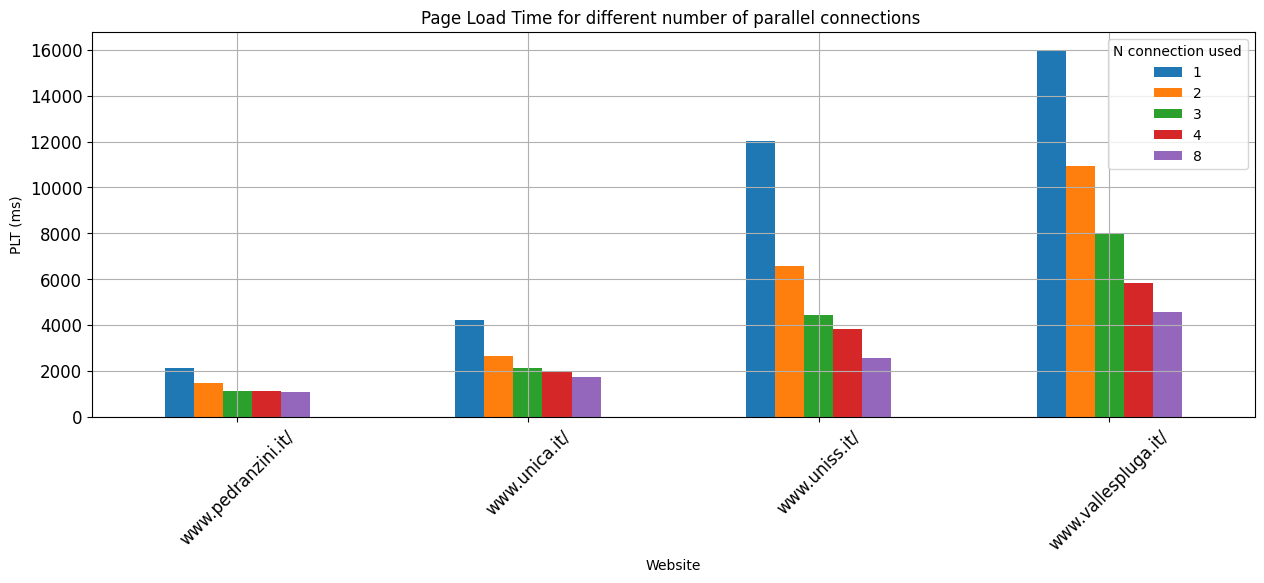
\includegraphics[width=\columnwidth]{images/plt_vs_conc_1.1.png}
  \caption{Page load time vs number of concurrent connections for different sites}
  \label{fig-1}
\end{figure}

\pagestyle{OtherPage}
\subsection{Impact of caching policies on PLTs}
\subsubsection*{Analyze and discuss the impacts of caching policies implemented by different
  commercial/institutional websites on the Page Load Times. Consider websites that support
  HTTP/1.1, HTTP/2 and HTTP/3 (possibly with unsecure and secure connections). Did you notice
  any expected or unexpected behavior?}


\begin{figure}[H]
  \centering
  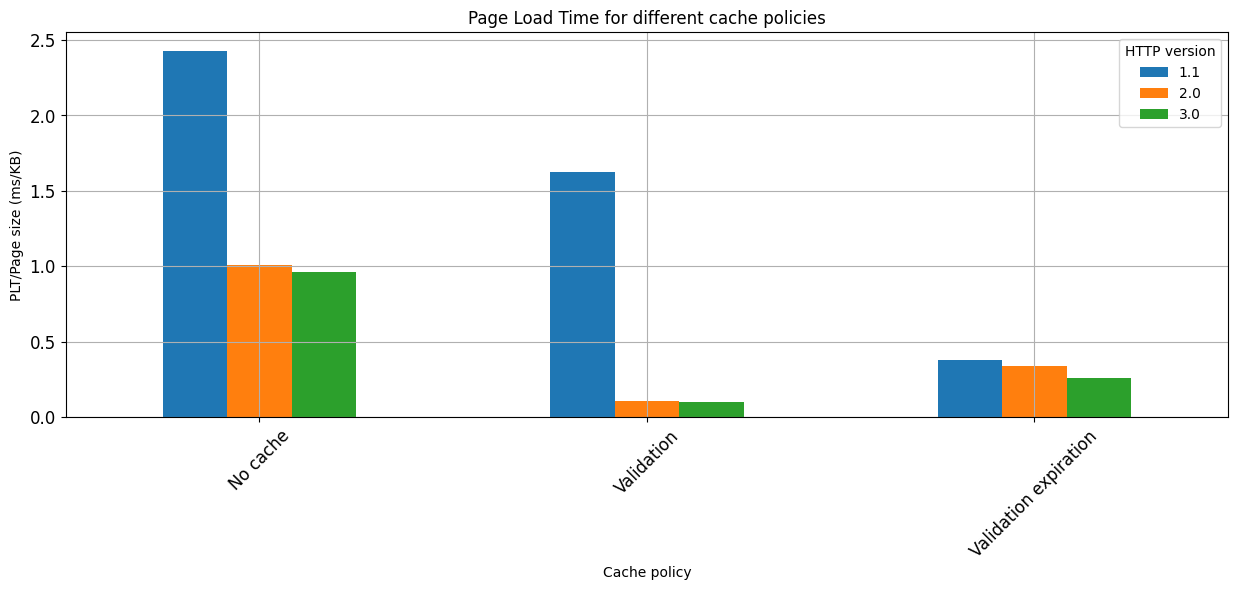
\includegraphics[width=\columnwidth]{images/plt_cache_policy.png}
  \caption{Page load time over page size for different cache policies for different HTTP versions}
  \label{fig-2}
\end{figure}

\subsection{Performance analisys using  Apache HTTP server benchmarking tool}
\subsubsection*{Analyze and discuss the performance of different commercial/institutional websites obtained
  under different conditions using the ab – Apache HTTP server benchmarking tool. Did you
  notice any expected or unexpected behavior?}

\begin{figure}[H]
  \centering
  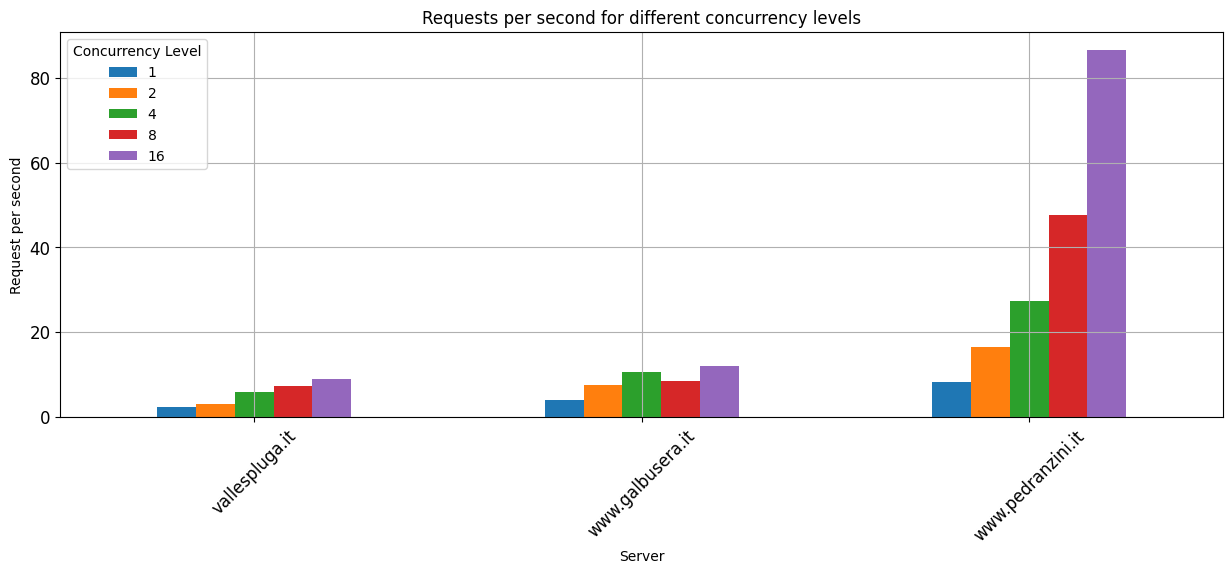
\includegraphics[width=\columnwidth]{images/Request_per_second_diff_conc.png}
  \caption{Number of request per second for different number of concurrent connections for different sites}
  \label{fig-3}
\end{figure}

\begin{figure}[H]
  \centering
  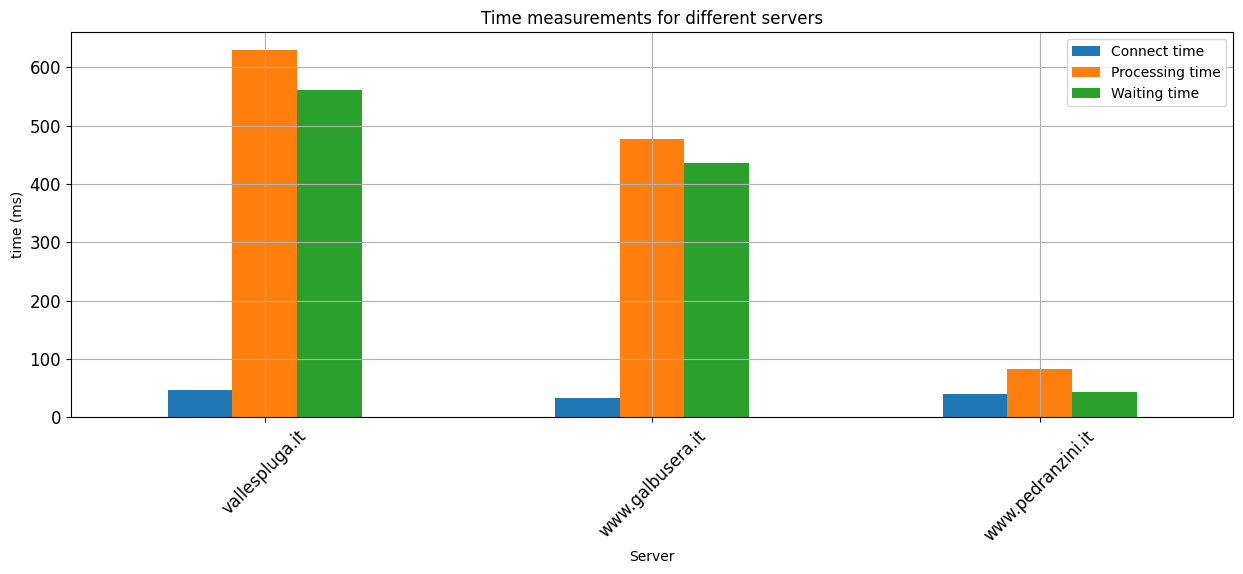
\includegraphics[width=\columnwidth]{images/time_diff_server.png}
  \caption{Time spent for the connection, for processing and for waiting for different sites}
  \label{fig-4}
\end{figure}

\begin{figure}[H]
  \centering
  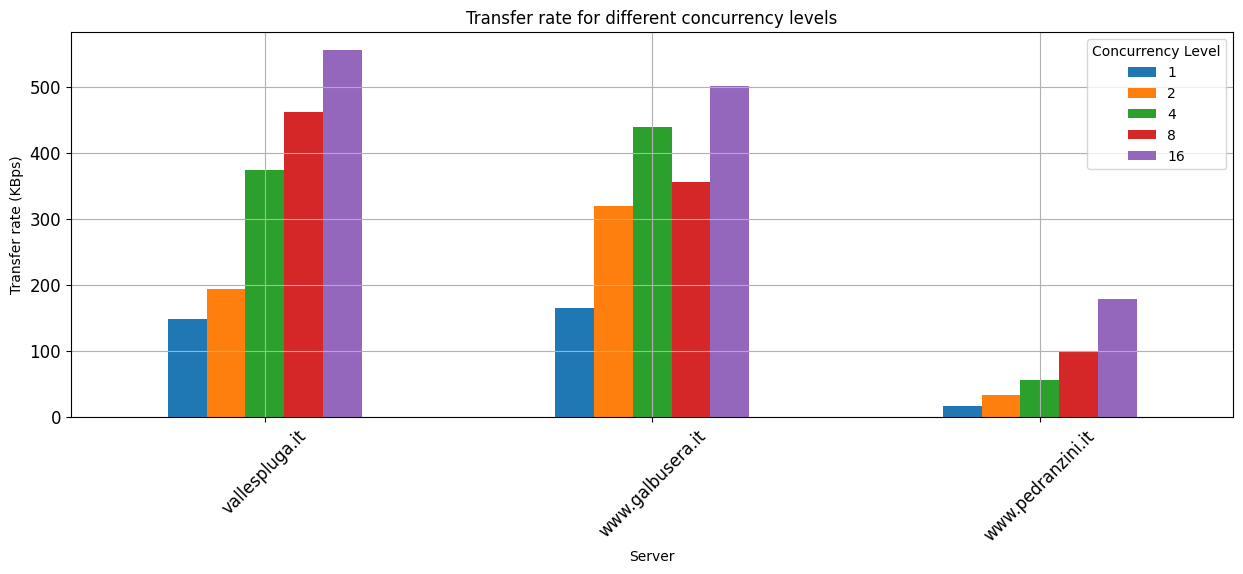
\includegraphics[width=\columnwidth]{images/transf_diff_conc.png}
  \caption{Transfer rate for different number of concurrent connections for different sites}
  \label{fig-5}
\end{figure}
\subsection{Performance analisys using h2load}
\subsubsection*{Analyze and discuss the performance of different commercial/institutional websites obtained
  under different conditions using the nghttp and h2load tools. In the experiments with
  h2load analyze the role of the warm-up time. Did you notice any expected or unexpected
  behavior?}

\begin{figure}[H]
  \centering
  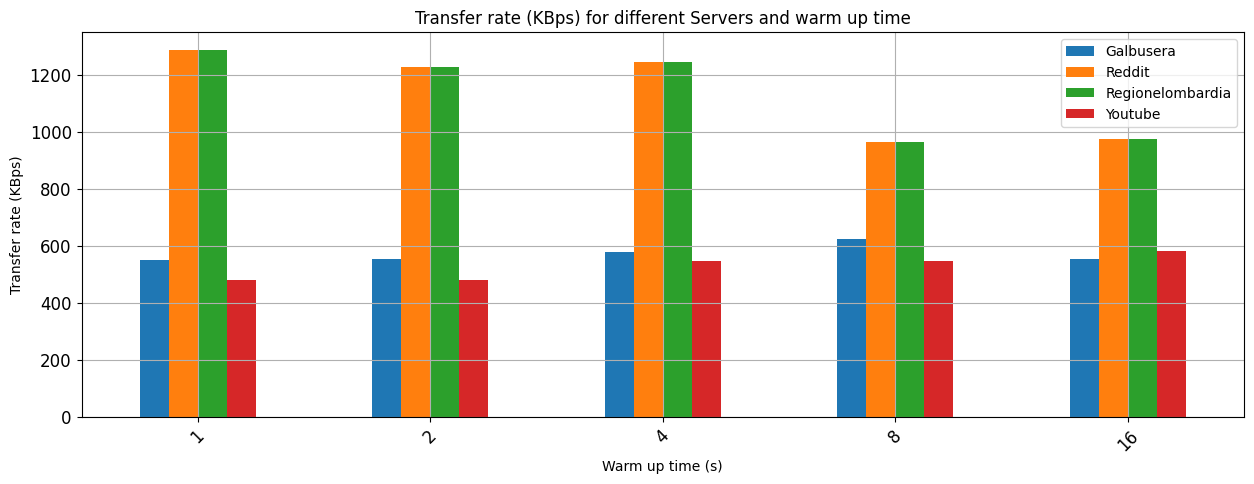
\includegraphics[width=\columnwidth]{images/transf_rate_diff_warm_up.png}
  \caption{Transfer rate for different warm up time for different sites}
  \label{fig-6}
\end{figure}

\begin{figure}[H]
  \centering
  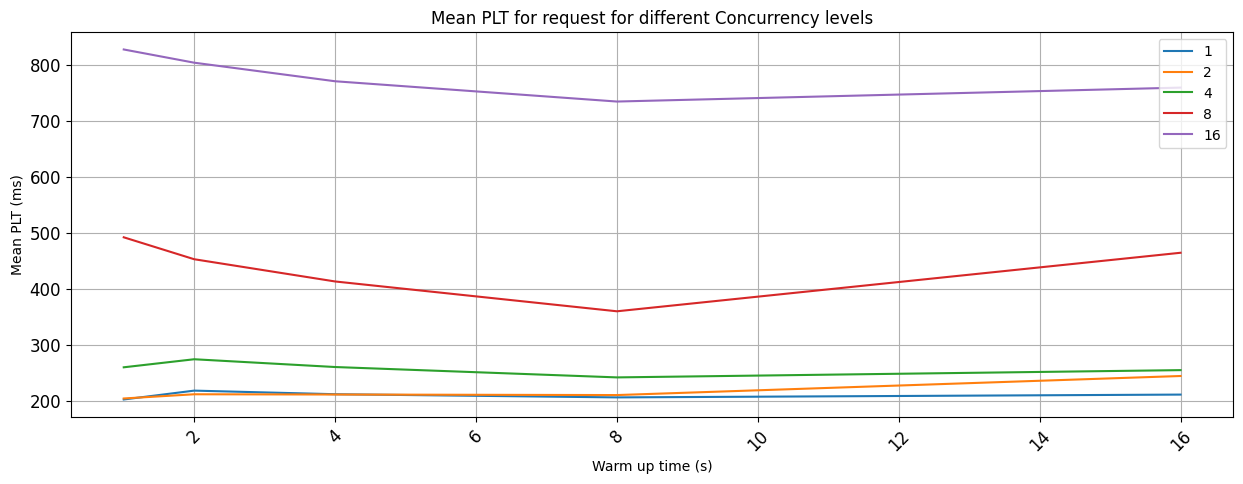
\includegraphics[width=\columnwidth]{images/mean_time_warm_up.png}
  \caption{mean time for different warm up time for different concurrent connections}
  \label{fig-7}
\end{figure}

\begin{figure}[H]
  \centering
  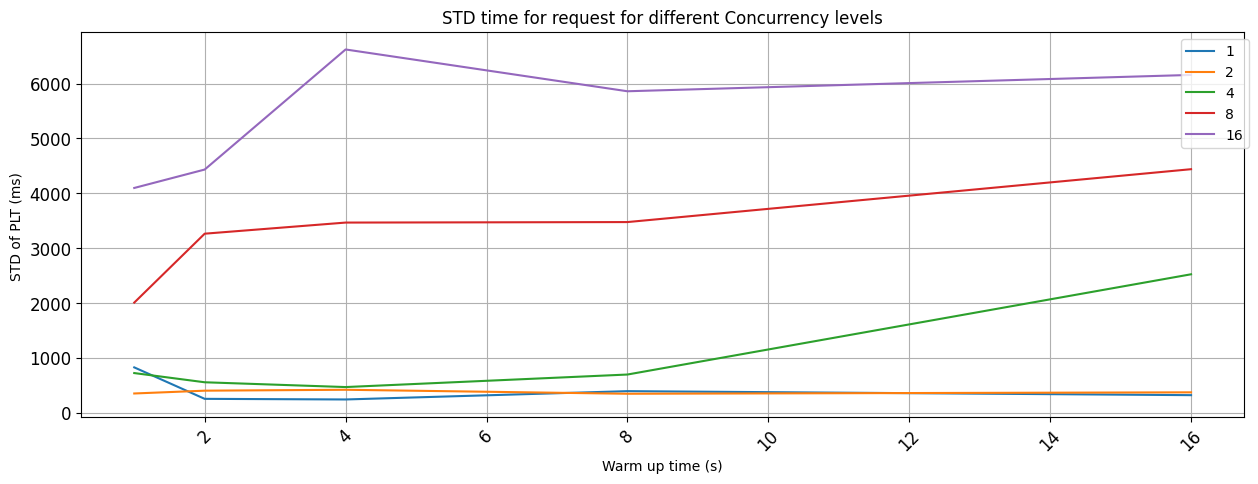
\includegraphics[width=\columnwidth]{images/var_warm_up.png}
  \caption{Standard deviation for different warm up time for different concurrent connections}
  \label{fig-8}
\end{figure}

\section{Conclusions}

\end{document}